\chapter{Разработка  Прототипа атомно-зондового томографа с лазерным испарением}\label{ch:ch2}


\section{Общая схема установки}\label{sec:ch2/sec1}

Как уже было сказано в первой главе наиболее значимым различием между конфигурациями установок АЗТ является выбранный тип испарения. Если используется сугубо полевой тип испарения, то появляется необходимость использовать различного рода системы компенсации энергий ионов. Это значительно усложняет разработку установки, а также требует наличия дополнительного узла и сложный расчет взаиморасположения образца, испаряющего контр-электрода, системы компенсации энергий ионов и детектирующей системы. Для разработки ПАЗЛ-3D \cite{scbibAPPLE} было выбрано испарение с помощью лазерной системы, для которого достаточно прямопролетной геометрии. Также прямо-пролетная геометрия обеспечивает в общем случае больший угол сбора данных, чем системы с рефлектроном (за исключением систем типа "сферическое зеркало"). Надо отметить, что выбор испарения с помощью лазера накладывает дополнительные требования по вводу лазерного излучения внутрь анализационного объема и взаиморасположения окна для лазера и образца, так как необходимо прямое попадание лазерного излучения на кончик образца.

Выбранная прямо-пролетная геометрия позволяет довольно легко оценить при разработке  разрешение по массе используя формулу \cref{eq:equation8}. Исходя из литературных данных (см. Глава \cref{sec:ch1/sec4}) диапазон возможных длин пролета ионов составляет от 11 до 25 см в Приложении \cref{app:A} были рассчитаны разрешения по массе для различных длин пролета. Ниже в Таблице \cref{tab:calcFWHM} для выбранного расстояния пролета в 180-185 мм приведены значения разрешения по массе для иона массой 30 а.е.м., с разбросом измерения времени пролета в 0,5 нс и в 1 нс. Оценка диапазона возможных разрешений по массе для разрабатываемого прибора была проведена при наименьшем и наибольшем из возможных разбросов времен пролета ионов. С учетом  стандартных комплектующих вакуумной системы установки, расстояние между кончиком образца и детектором в ПАЗЛ-3D было выбрано 183 мм.

\begin{table} [htbp]
	\centering
	\caption{Сравнение разрешения по массе для иона при различных ускоряющих напряжениях на образце}
	\label{tab:calcFWHM}
	\begin{SingleSpace}
		\begin{tabular} {| c | c | c | c |}
			\hline
			Длина пролета, мм & \thead{Разброс времени\\ пролета, нс} & Напряжение, кВ & \thead{Разрешение \\по массе, отн. ед.}  \\ \hline
			180-185 & 1 & 1  &  570               \\ \hline
			180-185 & 1 & 3  &  329               \\ \hline
			180-185 & 1 & 5  &  255               \\ \hline
			180-185 & 1 & 10 &  180               \\ \hline
			180-185 & 0,5 & 1  &  1140               \\ \hline
			180-185 & 0,5 & 3  &  658               \\ \hline
			180-185 & 0,5 & 5  &  510               \\ \hline
			180-185 & 0,5 & 10 &  360               \\ \hline
		\end{tabular}
	\end{SingleSpace}
\end{table}

Как видно из Таблицы \cref{tab:calcFWHM} установка АЗТ ПАЗЛ-3D в идеальных условия будет способна различать пики на масс-спектре отстоящие друг от друга на расстоянии от 0,01 а.е.м до 0,08 а.е.м. Такое качество масс-спектра более чем достаточно для распознания практически любых элементов и их изотопов. Полученное разрешение по массе соответствует разрешению по массе зарубежных установок аналогичной конфигурации. На Рисунке \cref{fig:main_scheme} представлена общая схема расположения образца, детектирующей системы, криогенной системы и лазерной системы в ПАЗЛ-3D.

\begin{figure}[htb]
	\centerfloat{
		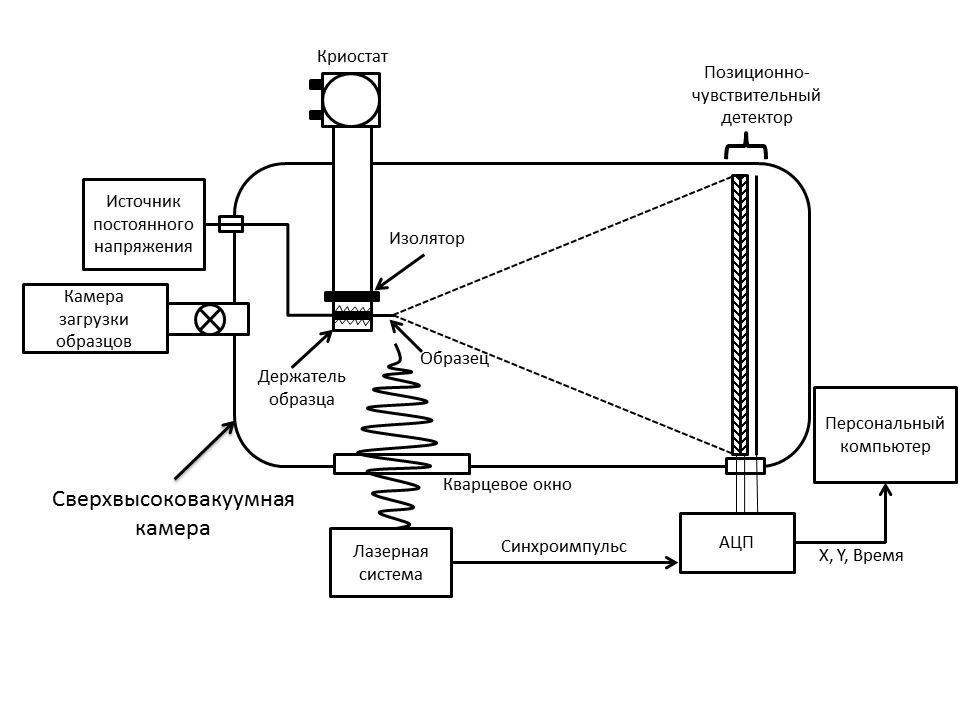
\includegraphics[width=\textwidth]{main_scheme}
	}
	\caption{Схема прототипа атомного зонда ПАЗЛ-3D с лазерным испарением и детектором на линиях задержки}
	\label{fig:main_scheme}
\end{figure}
  
Другой особенностью прямо-пролетной схемы установки можно назвать использование простых алгоритмов восстановления данных. Поскольку в приборе отсутствуют системы отклонения ионов, то траектории пролета можно рассчитывать не прибегая к сложным вычислениям электрических полей на пути пролета иона. Данная особенность важна, когда установка разрабатывается впервые и необходимо её максимально упростить для тестирования и апробирования общей концепции.

Для проектирования компоновки вакуумных объемов и деталей держателя образцов использовалась система автоматизированного проектирования (САПР) CATIA Dassault Systemes (Франция). К преимуществам данной системы можно отнести: одно из лучших ядер 3D, возможность быстро и удобно оперировать сборками в сотни деталей и наличие большого количества учебных материалов и пособий. Ниже на Рисунке \cref{fig:APPLE_CAD} показан схематический вид установки.
\begin{figure}[htb]
	\centerfloat{
		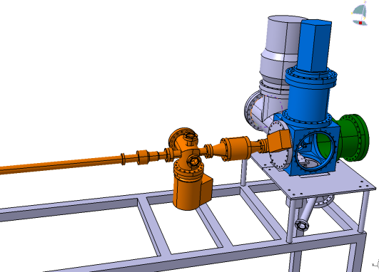
\includegraphics[width=\textwidth]{APPLE_CAD}
	}
	\caption{Внешний вид установки ПАЗЛ-3D в системе САПР CATIA на одном из этапов разработки. Оранжевым цветом выделена камера загрузки с транспортным штоком и шибером, синий - криосистема и часть анализационного объема, зеленый - фланец с расположенной внутри вакуумной частью детектирующей системы}
	\label{fig:APPLE_CAD}
\end{figure}

Как и любой современный микроскоп или томограф АЗТ нуждается в специальном программном обеспечении. Причем необходима разработка собственного ПО управления установкой и сбора на ней данных, так как разрабатываемая установка имеет отличные от зарубежных аналогов узлы. Также наиболее оптимальным решением является разработка собственного ПО для восстановления данных.


\FloatBarrier

\section{Вакуумная и криогенная системы}\label{sec:ch2/sec2}

Одна из основных и важнейших систем в атомно-зондовом томографе - вакуумная система. В АЗТ необходимо поддерживать сверхвысокий вакуум для работы детектора и для того, чтобы отсутствовали эффекты взаимодействия испаренных ионов с остаточным газом. В общем случае чем выше вакуум создает система, тем лучше. Минимально необходимый уровень вакуума считается равным $10^{-7}$ Торр. Но обычно стараются поддерживать от $10^{-9}$ Торр для уменьшения уровня детектируемого шума. Для некоторых материалов уровень вакуума критически важен, например, для исследования образцов, в составе которых есть водород или титан.

Ввиду необходимости высокого вакуума система имеет 2 камеры: загрузочную и анализационную. Анализационная камера находится всегда в откаченном состоянии. Откачка вакуумных объемов производится с помощью двух и трех ступенчатых систем насосов. В установке ПАЗЛ-3D форвакуумная часть системы представлена двумя спиральными сухими насосами Edwards XS35 (Великобритания), которые обеспечивают разрежение порядка $10^{-3}$ Торр. Далее на загрузочной камере высокий вакуум обеспечивается турбомолекулярным насосом Pfeiffer Vacuum HiPace 300. Уровень вакуума в загрузочной камере находится в пределах от $10^{-7}$ до $10^{-9}$ Торр. Откачку анализационного объема обеспечивают два последовательно установленных турбомолекулярных насоса Pfeiffer Vacuum HiPace 80 и Pfeiffer Vacuum HiPace 1200 (Германия), которые позволяют поддерживать вакуум до $10^{-11}$ Торр (при включенной криогенной системе). На Рисунке \cref{fig:APPLE_foto_main} представлен внешний вид установки ПАЗЛЗ-3D. Измерение уровня вакуума производится с помощью вакуумметров Thyracont VSH (Германия).

\begin{figure}[htb]
	\centerfloat{
		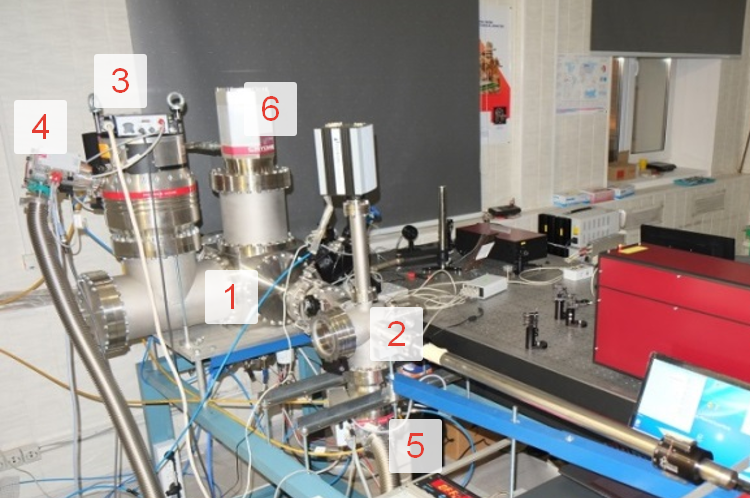
\includegraphics[width=\textwidth]{APPLE_foto_main}
	}
	\caption{Внешний вид установки ПАЗЛ-3D. 1 - анализационный объем, 2 - загрузочная камера, 3 - турбомолекулярный насос Pfieffer Vacuum HiPace 1200, 4 - турбомолекулярный насос Pfieffer Vacuum HiPace 80, 5 - турбомолекулярный насос Pfieffer Vacuum HiPace 300, 6 - криогенная система CryoMech PT805}
	\label{fig:APPLE_foto_main}
\end{figure}

\FloatBarrier
В качестве криогенной системы выбрана двух-ступенчатая криоголова CryoMech PT805 (США) типа <<пульсационная труба>>. Мощность первой ступени составляет 8 Вт при 20 К, мощность второй ступени 40 Вт при 80 К. Криосистема способна обеспечить минимальную температур 8 К. Но ввиду того, что между криосистемой и образцом находятся держатель патрона образца и монтажные медные проставки, то минимальная температура на образце составляет 20 К. На Рисунке \cref{fig:APPLE_cryosystem} показана криосистема вместе с держателем образца и криоголовой.

\begin{figure}[htb]
	\centerfloat{
		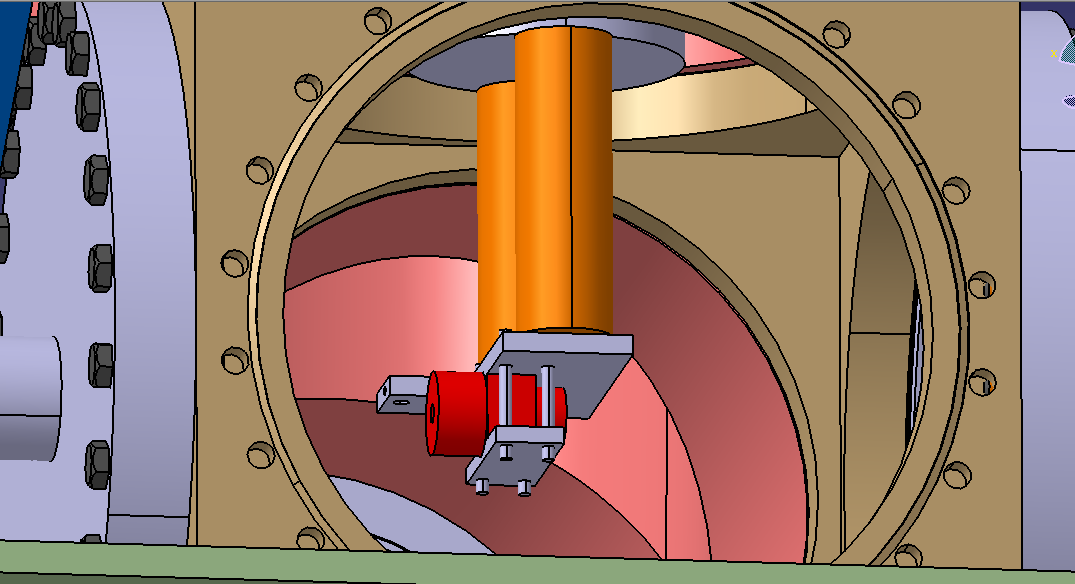
\includegraphics[width=\textwidth]{APPLE_cryoholder}
	}
	\caption{Изображение криоголовы и держателя образца в САПР}
	\label{fig:APPLE_cryosystem}
\end{figure}

\FloatBarrier

\section{Система испарения}\label{sec:ch2/sec3}

Как было выше сказано, для ПАЗЛ-3D было выбрано лазерное испарение. Соответственно, была изготовлена специальная лазерная система TETA~25ST производства ООО <<Авеста-Проект>> (Россия), состоящая из нескольких модулей. Основной блок лазера генерирует излучение с длиной волны 1030 нм и длительностью импульса 300 фс. Полная мощность лазерной системы составляет 3 Вт. Энергия импульса составляет от 0,1 до 250 мкДж. Частота работы системы составляет 50 кГц. На Рисунке \cref{fig:APPLE_lasersystem} показа схема лазерной системы.

\begin{figure}[htb]
	\centerfloat{
		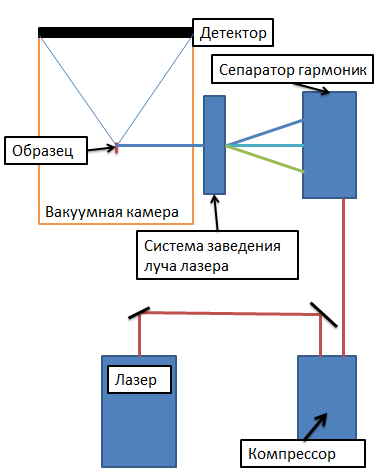
\includegraphics[width=.6\textwidth]{APPLE_lasersystem_2}
	}
	\caption{Схема лазерной системы ПАЗЛ-3D}
	\label{fig:APPLE_lasersystem}
\end{figure}

В системе используется капиллярный компрессор лазерных импульсов. Его принцип работы заключается в уширении спектра входящего лазерного импульса при его распространении в кварцевом капилляре, заполненном инертным газом ксеноном. В дальнейшем спектрально-уширенный импульс сжимается по времени при многократном отражении от чирпированных зеркал. Чирпированное зеркало представляет собой зеркало с многослойным диэлектрическим покрытием, при отражении от которого возникает задержка во времени для импульса с различными длинами волн. После компрессора длительность импульса может составлять от 30 до 60 фс в зависимости от настройки. Далее лазерное излучение опадает в сепаратор гармоник, где происходит генерация второй (515 нм), третьей (343 нм) или четвертой (257 нм) гармоник. Вторая гармоника имеет наибольшую мощность, что позволяет исследовать материалы при более широком диапазоне возможных энергий импульса. Третья и четвертая гармоники используются для получения более качественных данных при исследовании диэлектриков и полупроводников \cite{Gault06}.

Для испарения атомов (ионов) на образец подается постоянное напряжение с помощью источника высоковольтного напряжения марки FuG Electronik GmbH (до 13 кВ). Лазерное излучение фокусируется с помощью системы линз на кончик образца-иглы. Луч лазера заводится в камеру исследования с помощью системы зеркал и шаговых двигателей, обеспечивающей точность позиционирования менее 2 мкм. Введение лазерного луча в вакуумный объем проводится через специальное кварцевое окно с коэффициентом пропускания более 99\% для любой из 3-х гармоник. Также лазерная система генерирует синхроимпульс для измерения времени пролета частиц, который далее подается на вход модуля АЦП в детектирующей системе.


\FloatBarrier

\section{Детектирующая система}\label{sec:ch2/sec4}

В качестве базового варианта был выбран детектор производства RoentDek GmbH DLD120 с эффективным диаметром 120 мм. Детектирующая система состоит из сборки микроканальных пластин (МКП) и системы анодов, усилителя сигнала с детектора и аналого-цифрового преобразователя (АЦП) для оцифровки и передачи данных на компьютер. Схематичное изображение и принцип формирования сигнала при детектировании столкновения иона показан на Рисунке \cref{fig:APPLE_detectionsystem}. Оцифровка проводится с частотой дискретизации 5 ГГц для сигнала с МКП и с частотой 1 ГГц для сигналов с анодов. 

Принцип детектирования \cite{Spillman00} основан на линиях задержки и состоит в следующем. Ускоренный в поле вблизи образца ион попадает в канал МКП, порождает облако электронов, далее электроны попадают на систему анодов, наводя в проволоке анодов ЭДС. Затем сигнал усиливается в модуле усиления и передается на АЦП. Положение точки удара иона в МКП определяется по разнице времён прихода сигнала на концы соответствующего анода. 

\begin{figure}[ht]
	\begin{minipage}[b]{0.49\textwidth}\centering
		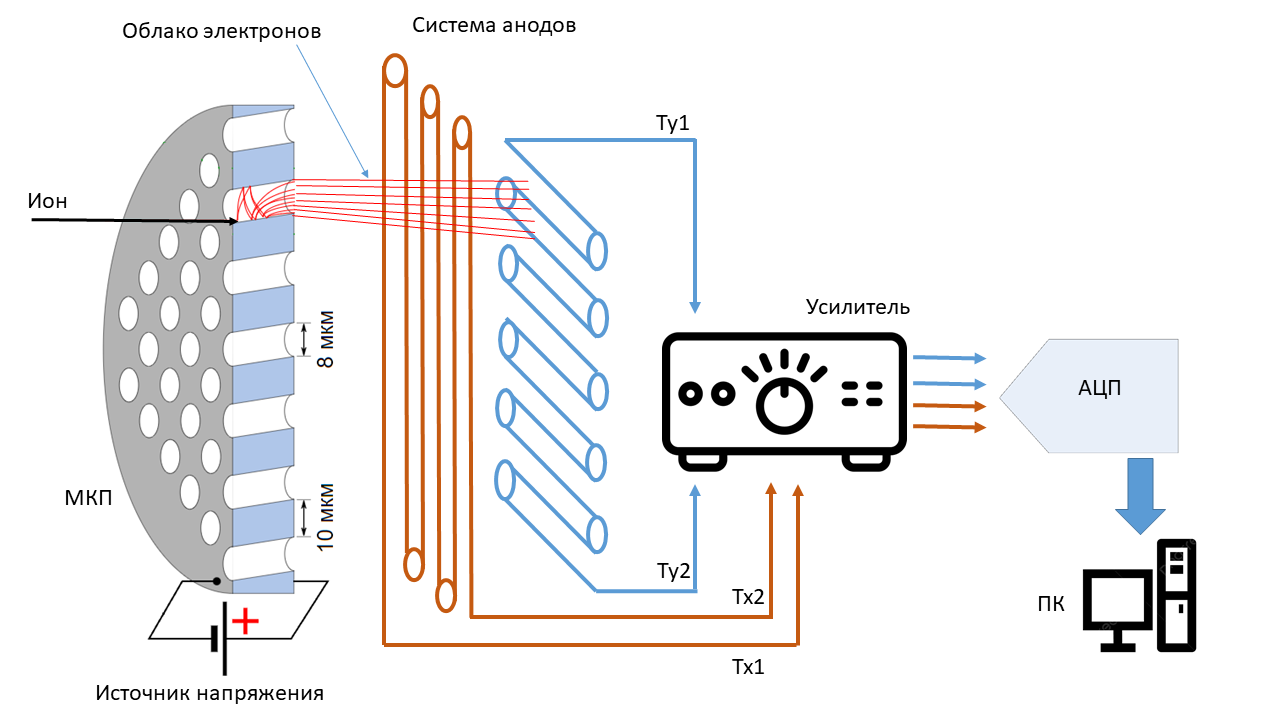
\includegraphics[width=\textwidth]{APPLE_detectionsystem} \\ а)
	\end{minipage}
	\begin{minipage}[b]{0.49\textwidth}\centering
		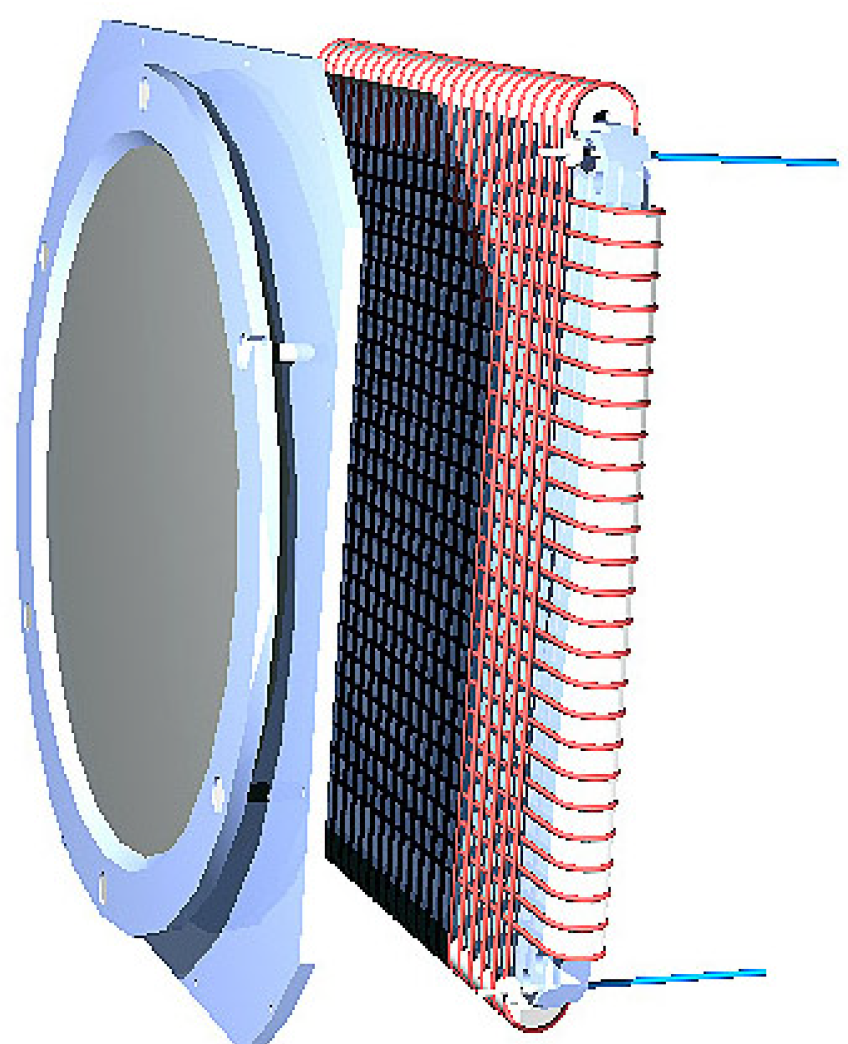
\includegraphics[width=\textwidth]{APPLE_detector} \\ б)
	\end{minipage}
	\caption{Схема работы детектирующей системы. а) Вверху показано столкновение иона с МКП, затем в МКП образуется облако электронов. Ниже показано, как падающее на аноды облако электронов формирует сигнал на выходе. б) Схематичное изображение детектирующей сборки МКП и анодов.}
	\label{fig:APPLE_detectionsystem}
\end{figure}


Координаты прилета частиц на детекторе определяются с точностью менее 100 мкм, что позволяет обеспечить пространственное разрешение прототипа, близкое к атомарному (область образца с характерным размером 100 нм ставится в соответствие области детектора 120 мм). Имеющаяся эффективная площадь детектора в 120 мм при длине пролета ионов 183 мм позволяет достичь угла сбора данных 32$^{\circ}$, что сопоставимо с аналогичными установками.

\FloatBarrier

\section{Программное обеспечение для управления сбором атомно-зондовых данных}\label{sec:ch2/sec5}

Для сбора данных с детектирующей системы разработано и создано специализированное программное обеспечение <<ПАЗЛ-3D-Сбор V 1.0>> \cite{SBOR}. Данное ПО решает задачи по сбору данных от АЦП детектирующей системы по USB соединению, управляет напряжением на образце по последовательному интерфейсу RS-232. Данные сохраняются в специализированном формате данных *.pos. На графическом интерфейсе ПО пользователь может наблюдать в реальном времени графики напряжения, потока событий на детекторе, предварительный масс-спектр исследуемого образца. Данное ПО работает на персональном компьютере под управлением операционной системы Windows. Разработано ПО в среде разработки Visual Studio с использованием библиотек Qt5 и других библиотек, необходимых для взаимодействия с АЦП и с источником напряжения ПАЗЛ-3D. Внешний вид окна программы сбора данных представлен на рисунке \cref{fig:APPLE_sbor}.

\begin{figure}[htb]
	\centerfloat{
		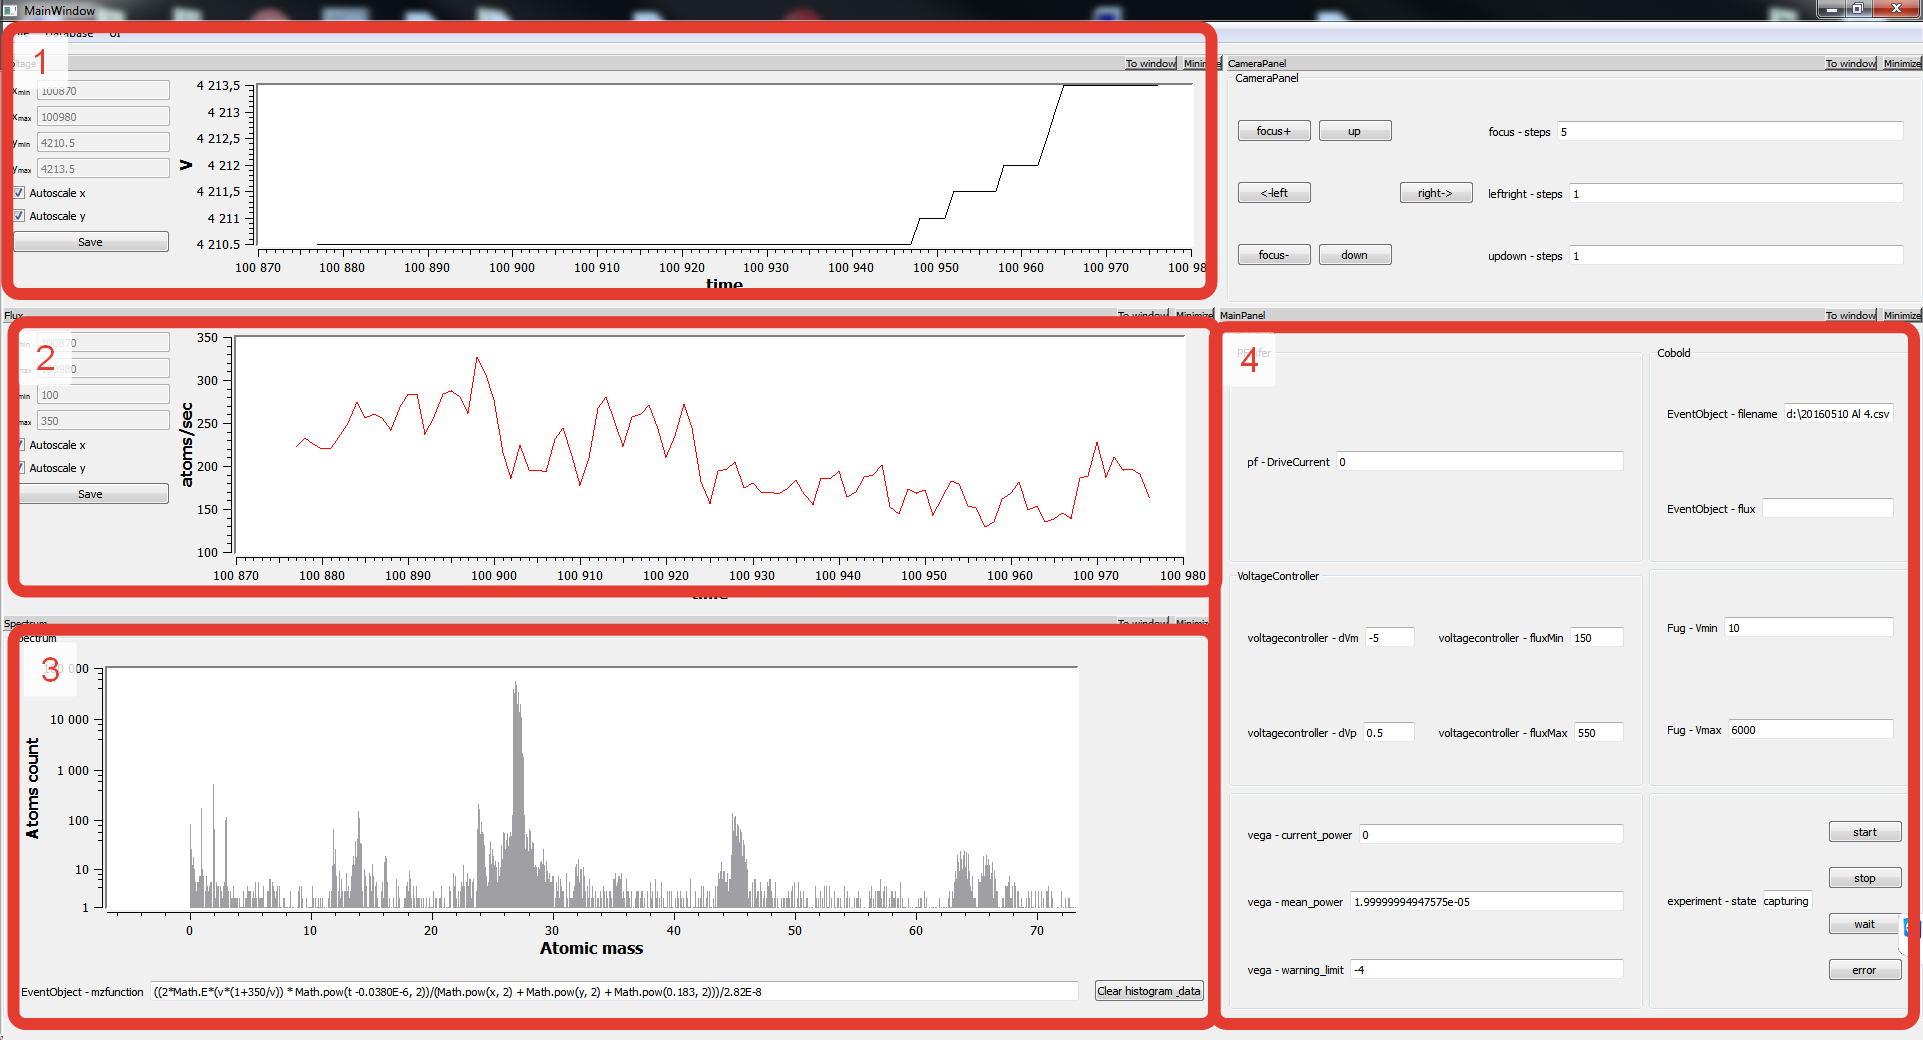
\includegraphics[width=\textwidth]{APPLE_sbor}
	}
	\caption{Внешний вид пользовательского интерфейса программы сбора данных  <<ПАЗЛ-3D-Сбор V 1.0>>, 1 - график напряжения на образце, 2 - график потока событий на детектирующей системе, 3 - предварительный масс-спектр, 4 - настройки и управление}
	\label{fig:APPLE_sbor}
\end{figure}

Восстановление и обработка данных проводится в специально разработанном ПО <<КВАНТМ-3D>> \cite{KVANTM}. Из отличительных особенностей данной программы стоит отметить возможность многопоточных вычислений, сопряжение с базой данных исследований, возможность проведения части расчетов на графических процессорах (GPU) и возможность пакетной обработки данных. Графический интерфейс программы позволяет визуализировать трехмерные карты распределения атомов в образец, строить масс-спектры, графики (линейные концентрации, различные распределения в методах анализа неоднородностей материалов), строить дву-мерные карты распределения концентраций или плотностей элементов, управлять параметрами восстановления и анализа данных. На рисунке \cref{fig:APPLE_kvant} показан внешний вид интерфейса программы обработки данных.

\begin{figure}[htb]
	\centerfloat{
		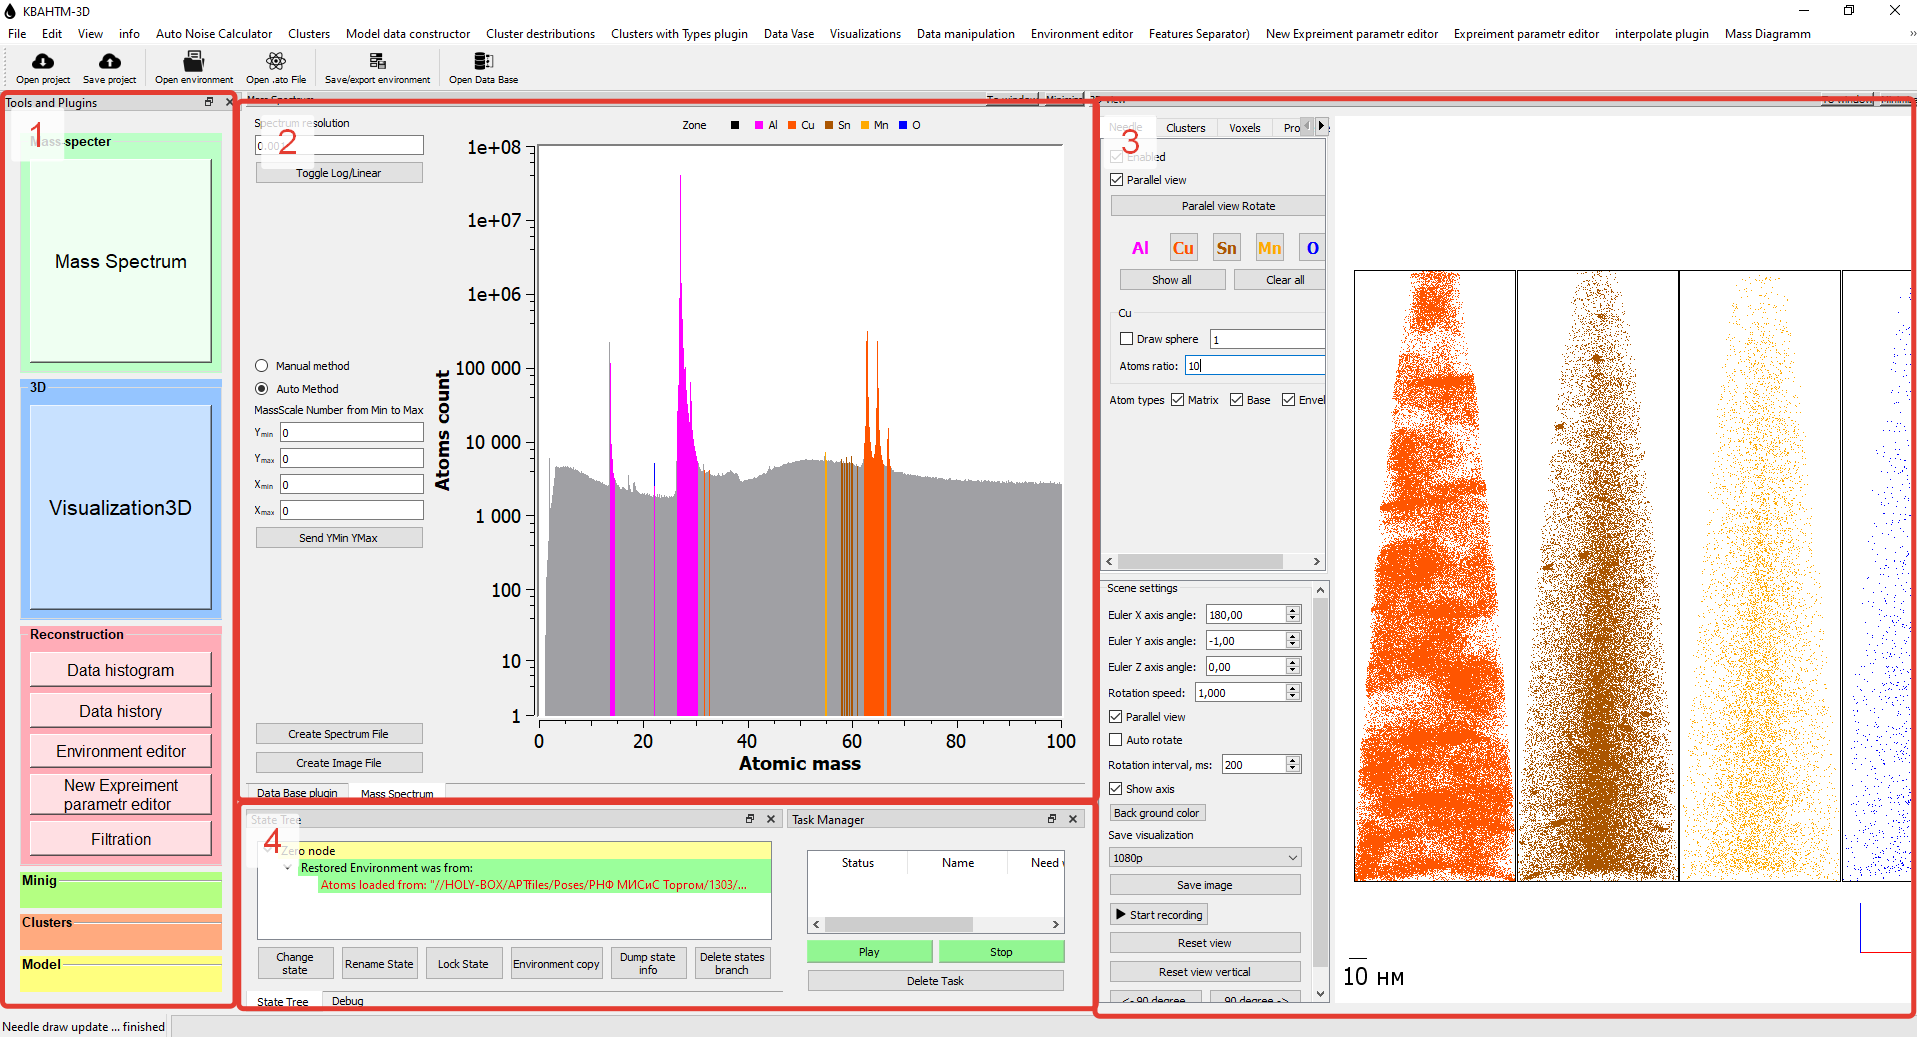
\includegraphics[width=\textwidth]{APPLE_kvant}
	}
	\caption{Внешний вид пользовательского интерфейса программы обработки данных <<КВАНТМ-3D>>, 1 - панель инструментов восстановления и анализа данных, 2 - масс-спектр образца, 3 - трехмерные атомные карты распределения химических элементов, 4 - управление состояниями и очередью процессов в программе}
	\label{fig:APPLE_kvant}
\end{figure}

Восстановление масс-спектра проводится по формуле \cref{eq:equation8}, с дополнительной оптимизацией Шутова \cite{Shutov19}. Трехмерные координаты восстанавливаются по специальному алгоритму, основанному на алгоритме, предложенным группой под руководством Bas \cite{Bas95}. В <<КВАНТМ-3D>> реализованы основные инструменты анализа атомно-зондовых данных:

\begin{itemize}
	\item Состав образца,
	\item Линейные концентрации,
	\item Поиск кластеров методом максимального разделения (Maximum separation method MSM),
	\item Поиск кластеров по ближайшим соседям (KNN),
	\item Парно-корреляционный анализ (парно-корреляционная функция pair-correlation function PCF),
	\item Анализ распределения ближайших соседей (KNN),
	\item Построение поверхностный одинаковой концентрации (изо-концентрационные поверхности - изо-поверхности),
	\item Построение гистограмм близости (proximity histograms - proxigrams),
	\item Построение двумерных карт плотности.
\end{itemize}

\FloatBarrier
\section{Разработка системы автоматизации управления атомно-зондовым томографом ПАЗЛ-3D}\label{sec:ch2/sec6}

Рабочими узлами атомно-зондового томографа являются довольно сложные, с точки зрения управления, системы: вакуумная, высоковольтного питания, перемещения образца, бесперебойного питания и охлаждения образца. Некорректное управление ими может привести к повреждению и дорогостоящему ремонту. Для решения задач по минимизации возможных ошибок оператора, ведения детального журнала о состоянии установки и для автоматизации части процедур исследования и протоколов безопасности были разработаны средства контроля и автоматизации. 

К инструментам реализации системы автоматизации и контроля предъявлялись следующие требования: модульность, открытость исходного кода, масштабируемость и удобство разработки. В качестве языка программирования выбран объектно-ориентированный язык C$\#$, относящийся к семье языков с С-подобным синтаксисом, имеющим статическую типизацию, поддерживающий полиморфизм, перегрузку операторов, делегаты, атрибуты, события, свойства, переменные, обобщенные типы и методы, исключения. В качестве платформы для разработки была выбрана модульная платформа .NET, как одна из самых современных платформ для разработки с открытом исходным кодом. В качестве базы данных используется свободная реляционная система управления базами данных (СУБД) MySQL. Резервное копирование (репликация базы данных) проводится постоянно средствами СУБД MySQL. На Рисунке \cref{fig:auto_APPLE_manage}  показана схема взаимодействия пользователей и программных модулей между собой и АЗТ ПАЗЛ-3D.

\begin{figure}[htb]
	\centerfloat{
		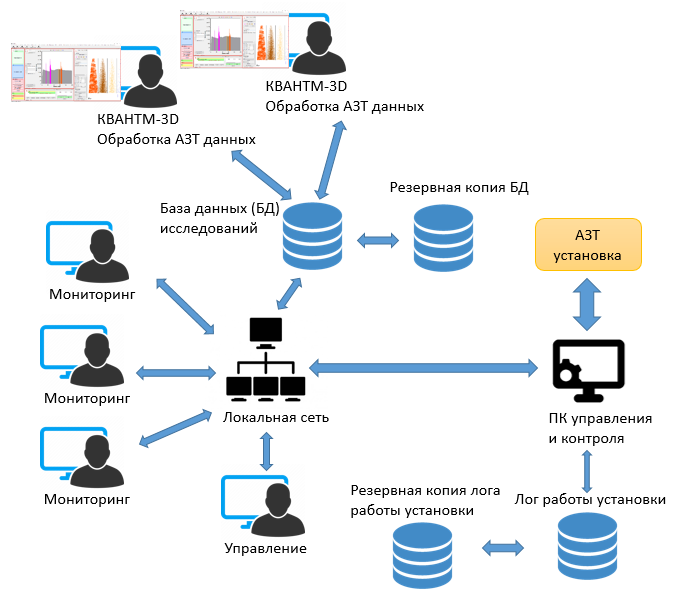
\includegraphics[width=.7\textwidth]{auto_APPLE_manage}
	}
	\caption{Схема управления и мониторинга работы атомно-зондового томографа ПАЗЛ-3D}
	\label{fig:auto_APPLE_manage}
\end{figure}

Для управления узлами установки атомно-зондовой томографии ПАЗЛ-3D разработано программное обеспечение JabberWocky (ССЫЛКА). Данное ПО способно взаимодействовать с блоками управления турбомолекулряных насосов, источником напряжения, лазерной системой, клапанами, шибером, источником бесперебойного питания. Используется логика машины состояний, когда установка находится в одном из нескольких состояний, которые всё время сменяют друг друга. В используемой логике набор состояний и переходов предопределен (<<Детерминированный конечный автомат>>). Опрос узлов установки проводится непрерывно, с записью данных в локальные файлы логов и с отсылкой данных в программу мониторинга. Программа управления установкой АЗТ имеет API (application programming interface, интерфейс программирования приложения) для взаимодействия с программой сбора данных <<КВАНТМ-3D>>. Для мониторинга работы СУБД и ПО управления установкой АЗТ используется Loki - набор программ для хранения и индексации логов и Grafana - программная среда визуализации данных, ориентированная на данные систем мониторинга. На Рисунке \cref{fig:auto_APPLE_scheme} показана схема взаимодействия узлов ПАЗЛ-3D для автоматизации управления.

\begin{figure}[htb]
	\centerfloat{
		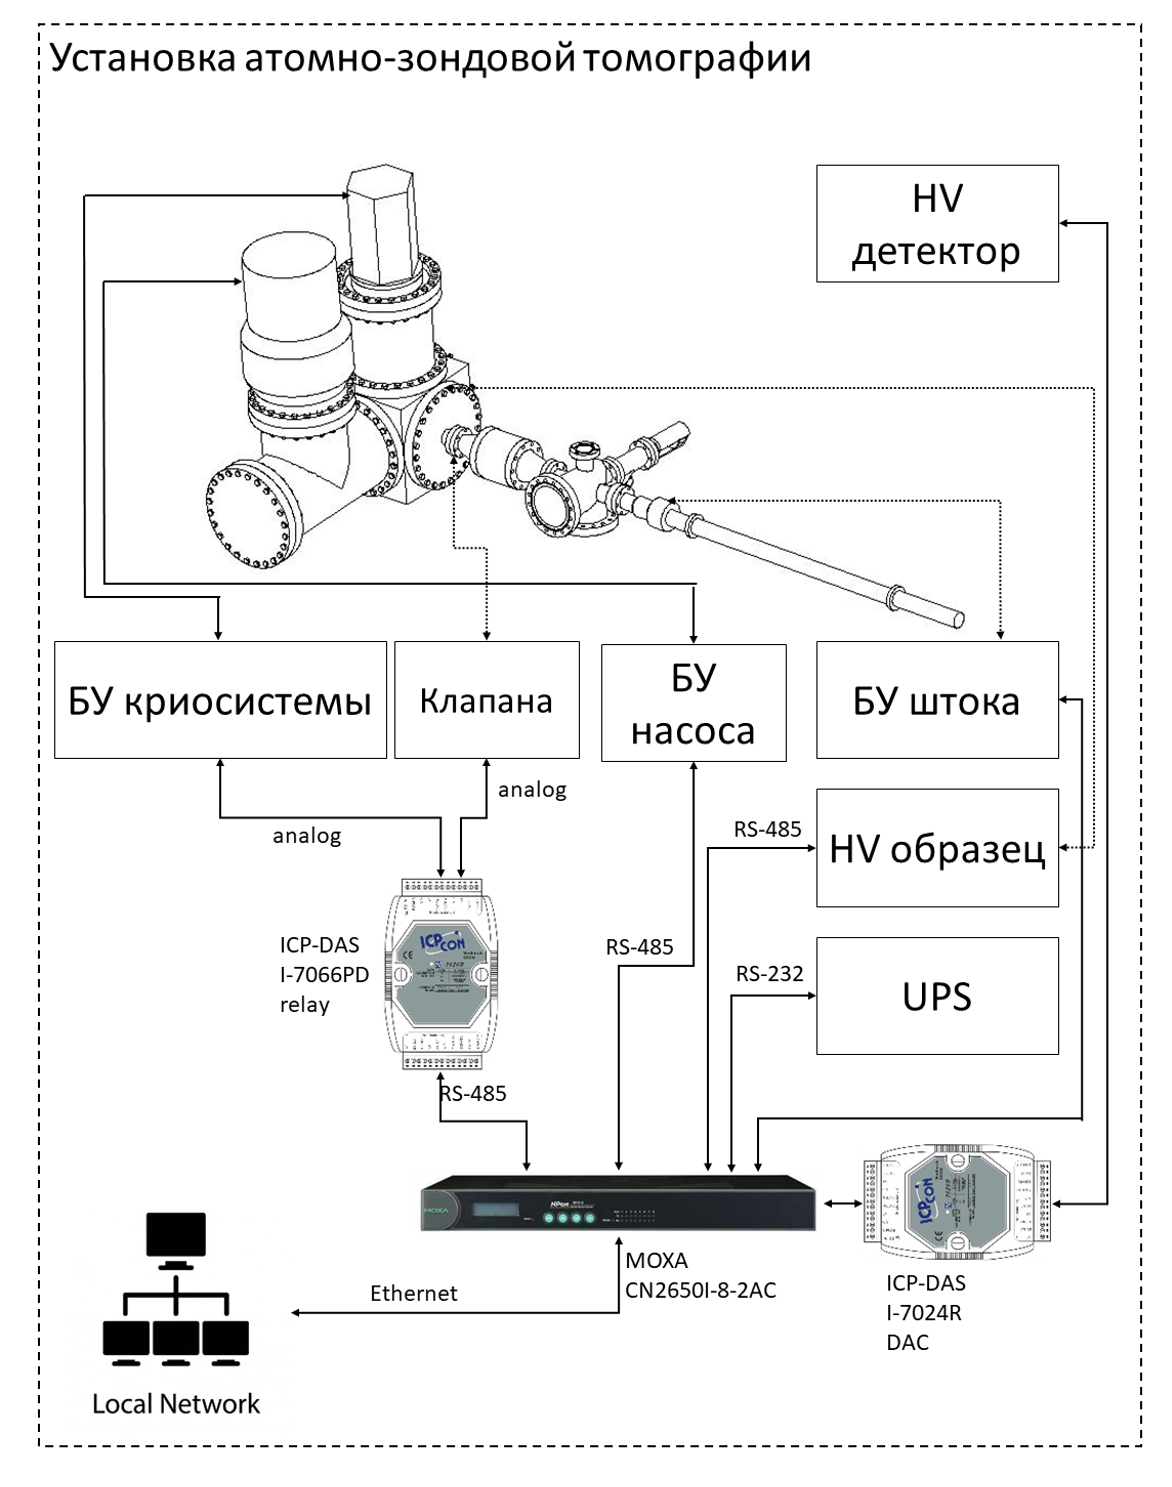
\includegraphics[width=.7\textwidth]{auto_APPLE_scheme}
	}
	\caption{Схема взаимодействия узлов ПАЗЛ-3D в рамках автоматизированной работы. HV детектор - источник напряжения для детектирующей системы, UPS - источник бесперебойного питания, HV образец - источник напряжения для образца, БУ - блок управления, Local Network - локальная сеть, MOXA CN2650I-8-2AC -конвертов интерфейсов RS-232-422/485 в Enthernet}
	\label{fig:auto_APPLE_scheme}
\end{figure}

\begin{figure}[htb]
	\centerfloat{
		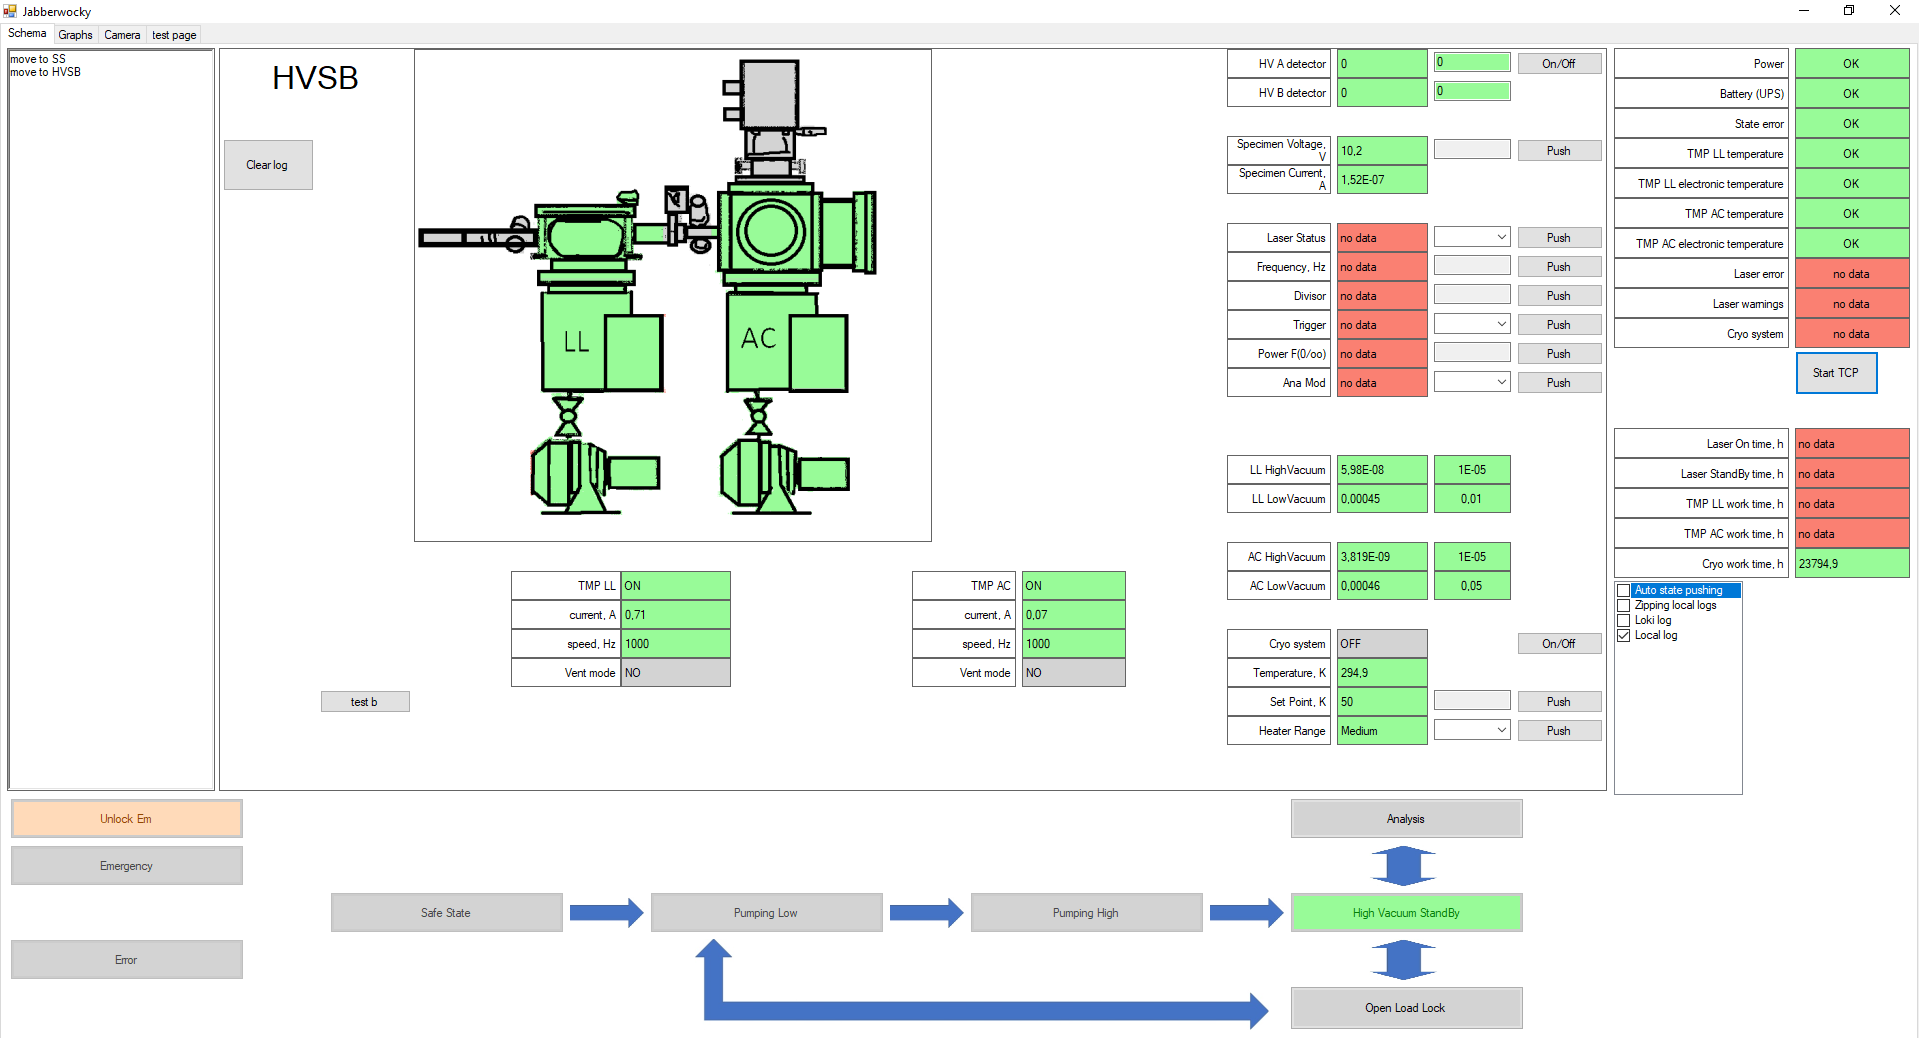
\includegraphics[width=.9\textwidth]{auto_APPLE_Jabber}
	}
	\caption{Внешний вид интерфейса ПО управления атомно-зондовым томографом}
	\label{fig:auto_APPLE_Jabber}
\end{figure}

Внешний вид интерфейса ПО управления атомно-зондовым томографом показан на Рисунке \cref{fig:auto_APPLE_Jabber}. В разработанной системе мониторинга и управления установкой АЗТ ПАЗЛ-3D можно отметить следующие  технологи и особенности архитектуры:

\begin{itemize}[beginpenalty=10000]
	\item С$\#$ (.NET), MySQL,
	\item Все списки команд и все настройки таймеров в файлах настроек JSON,
	\item Все переходы между состояниями заданы программно и зависят только от настоящего состояния системы и не могут быть изменены обычным пользователем,
	\item Подключение большинства узлов по RS-485/232,
	\item Удаленный доступ для мониторинга по локальной сети для нескольких пользователей (Клиент-серверное приложение),
	\item Сохранение записей на всех команд/изменений на стороне сервера и клиента,
	\item Данные исследований сохраняются в локальную базу данных с поддержкой резервного копирования.
\end{itemize}


\FloatBarrier
\section{Основные результаты по главе 2}\label{sec:ch2/sec7}

В главе описана общая схема и концепция разработанного атомно-зондового томографа с лазерным испарением ПАЗЛ-3D. Благодаря использованию современного фемтосекнундного лазера в России появилась возможность исследовать широкий спектр материалов, в том числе алюминиевые сплавы, полупроводящие и диэлектрические материалы. Основные технические характеристики показаны в Таблице \cref{tab:APPLEcharac}.

\begin{table} [htbp]
	\centering
	\caption{Технические и эксплуатационные характеристики установки ПАЗЛ-3D}
	\label{tab:APPLEcharac}
	\begin{SingleSpace}
		\begin{tabular} {| c | c |}
			\hline
			Наименование параметра & Значение  \\ \hline
			Температура образца & 22-70 К                \\ \hline
			Напряжение на образце & 1-10,5 кВ               \\ \hline
			Скорость сбора данных & 1 - 5 тыс. событий/сек                \\ \hline
			Вакуум & $<5*10^{-9}$ Торр                \\ \hline
			Длины волн лазера & 515, 343, 257 нм               \\ \hline
			Длительность импульса лазера & 30-300 фс               \\ \hline
			Частота воздействий лазера & 25-50 кГц                \\ \hline
			Габариты установки & 3х4 м               \\ \hline
			Эффективность детектирования & 60 \%              \\ \hline
			Временное разрешение детектора & 50 пс               \\ \hline
			Точность определения координат детектора  & 50 мкм               \\ \hline
		\end{tabular}
	\end{SingleSpace}
\end{table}
В ходе разработки получен уникальный опыт разработки в САПР комплексных установок,  работы с детекторами на основе линий задержки и проектирования многокомпонетной системы (аппаратная часть, программная часть и методическая часть). Успешная разработка АЗТ ПАЗЛ-3D позволила решить ряд задач:

\begin{itemize}
	\item Подтверждена работоспособность концепции атомно-зондового томографа с фемтосекундным лазерным испарением с прямопролетной геометрией детектирования частиц,
	\item Расширен круг исследуемых материалов с помощью АЗТ.
\end{itemize}

Проделанная работа по разработке делает возможным развитие таких направлений как:
\begin{itemize}
	\item Модернизация имеющихся АЗТ и разработка новых устанвоок АЗТ в интересах отечественных материаловедческих институтов (ВНИИНМ им. Бочвара, МИСИС, МИФИ  и др.),
	\item Развитие программного обеспечения для анализа микро- и наноструктуры материалов,
	\item Развитие направления создания цифровых карт материалов.
\end{itemize}

\FloatBarrier







